% Options for packages loaded elsewhere
\PassOptionsToPackage{unicode}{hyperref}
\PassOptionsToPackage{hyphens}{url}
%
\documentclass[
]{article}
\usepackage{amsmath,amssymb}
\usepackage{lmodern}
\usepackage{iftex}
\ifPDFTeX
  \usepackage[T1]{fontenc}
  \usepackage[utf8]{inputenc}
  \usepackage{textcomp} % provide euro and other symbols
\else % if luatex or xetex
  \usepackage{unicode-math}
  \defaultfontfeatures{Scale=MatchLowercase}
  \defaultfontfeatures[\rmfamily]{Ligatures=TeX,Scale=1}
\fi
% Use upquote if available, for straight quotes in verbatim environments
\IfFileExists{upquote.sty}{\usepackage{upquote}}{}
\IfFileExists{microtype.sty}{% use microtype if available
  \usepackage[]{microtype}
  \UseMicrotypeSet[protrusion]{basicmath} % disable protrusion for tt fonts
}{}
\makeatletter
\@ifundefined{KOMAClassName}{% if non-KOMA class
  \IfFileExists{parskip.sty}{%
    \usepackage{parskip}
  }{% else
    \setlength{\parindent}{0pt}
    \setlength{\parskip}{6pt plus 2pt minus 1pt}}
}{% if KOMA class
  \KOMAoptions{parskip=half}}
\makeatother
\usepackage{xcolor}
\usepackage[margin=1in]{geometry}
\usepackage{graphicx}
\makeatletter
\def\maxwidth{\ifdim\Gin@nat@width>\linewidth\linewidth\else\Gin@nat@width\fi}
\def\maxheight{\ifdim\Gin@nat@height>\textheight\textheight\else\Gin@nat@height\fi}
\makeatother
% Scale images if necessary, so that they will not overflow the page
% margins by default, and it is still possible to overwrite the defaults
% using explicit options in \includegraphics[width, height, ...]{}
\setkeys{Gin}{width=\maxwidth,height=\maxheight,keepaspectratio}
% Set default figure placement to htbp
\makeatletter
\def\fps@figure{htbp}
\makeatother
\setlength{\emergencystretch}{3em} % prevent overfull lines
\providecommand{\tightlist}{%
  \setlength{\itemsep}{0pt}\setlength{\parskip}{0pt}}
\setcounter{secnumdepth}{-\maxdimen} % remove section numbering
\ifLuaTeX
  \usepackage{selnolig}  % disable illegal ligatures
\fi
\IfFileExists{bookmark.sty}{\usepackage{bookmark}}{\usepackage{hyperref}}
\IfFileExists{xurl.sty}{\usepackage{xurl}}{} % add URL line breaks if available
\urlstyle{same} % disable monospaced font for URLs
\hypersetup{
  pdftitle={Tarea Empírica 2 - Macroeconometría},
  pdfauthor={Profesor: Mauricio Tejada - Estudiante: Matías Vicuña},
  hidelinks,
  pdfcreator={LaTeX via pandoc}}

\title{Tarea Empírica 2 - Macroeconometría}
\author{Profesor: Mauricio Tejada - Estudiante: Matías Vicuña}
\date{30/07/2022}

\begin{document}
\maketitle

\hypertarget{desarrollo}{%
\section{Desarrollo}\label{desarrollo}}

\hypertarget{pregunta-1}{%
\subsection{Pregunta 1}\label{pregunta-1}}

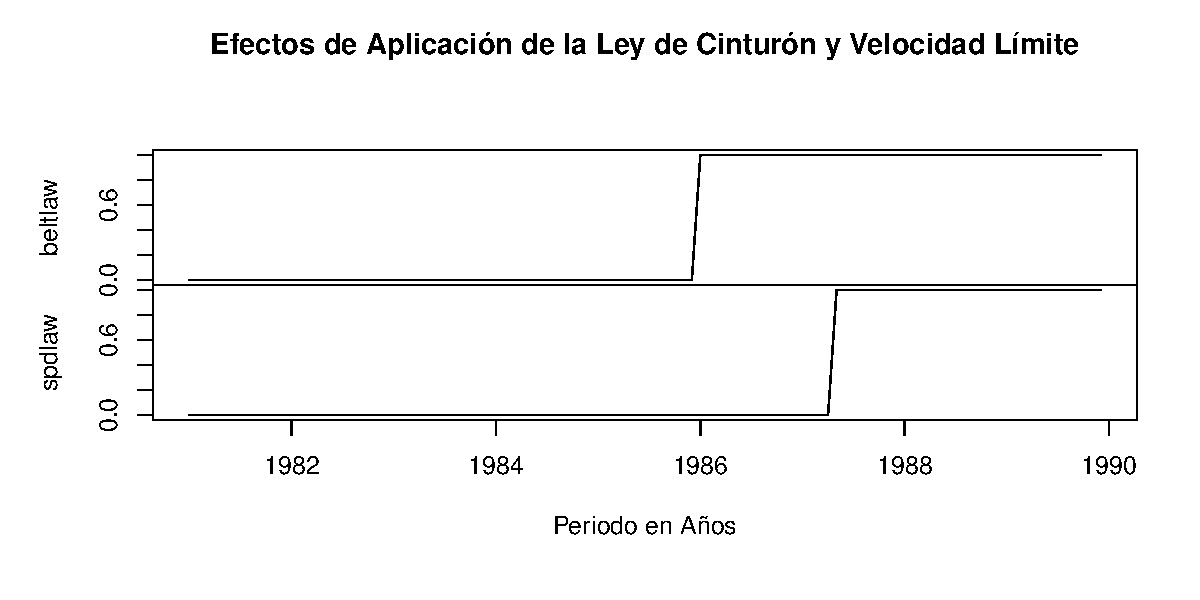
\includegraphics{Tarea-Empírica-2---Matías-Vicuña_files/figure-latex/P1 - Grafico-1.pdf}

Respuesta: se puede observar que la ley del cinturón de seguridad entró
en vigor en Diciembre de 1985, de ahí hasta Enero de 1986 se vió el
efecto de esta ley en vigor. En el caso de la ley de velocidad, esta se
aprecia que entro en vigor en Abril de 1987, en donde subió hasta Mayo
del mismo año.

\hypertarget{pregunta-2}{%
\subsection{Pregunta 2}\label{pregunta-2}}

\% Table created by stargazer v.5.2.3 by Marek Hlavac, Social Policy
Institute. E-mail: marek.hlavac at gmail.com \% Date and time: Tue, Aug
30, 2022 - 23:55:23

\begin{table}[!htbp] \centering 
  \caption{} 
  \label{} 
\begin{tabular}{@{\extracolsep{5pt}}lc} 
\\[-1.8ex]\hline 
\hline \\[-1.8ex] 
 & \multicolumn{1}{c}{\textit{Dependent variable:}} \\ 
\cline{2-2} 
\\[-1.8ex] & log(totacc) \\ 
\hline \\[-1.8ex] 
 Constant & 10.50$^{***}$ \\ 
  & (0.01) \\ 
  trend(db\_ts) & 0.03$^{***}$ \\ 
  & (0.002) \\ 
 \hline \\[-1.8ex] 
Observations & 108 \\ 
R$^{2}$ & 0.68 \\ 
\hline 
\hline \\[-1.8ex] 
\textit{Note:}  & \multicolumn{1}{r}{$^{*}$p$<$0.1; $^{**}$p$<$0.05; $^{***}$p$<$0.01} \\ 
\end{tabular} 
\end{table}

Respuesta: Corrigiendo por la tendencia que, el número de accidentes
totales en términos porcentuales se explican por la tendencia con un
aumento de aprox 3,4\%. siendo esta estadísticamente significativa con
99\% de confianza. He de decir también que el modelo contempla un
\(R^2\) significativo de 0,67 aproximadamente.

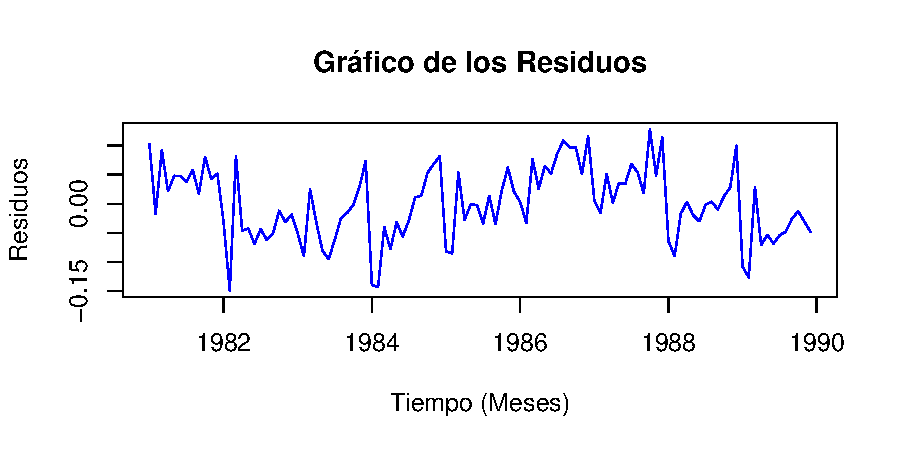
\includegraphics{Tarea-Empírica-2---Matías-Vicuña_files/figure-latex/Gráfica 2 de los Residuos-1.pdf}

Continuación Respuesta: Se aprecia en el gráfico de los residuos que no
hay una varianza ni un promedio constante, por lo cual la aletoriedad
del mismo modelo evidencia ciclos muy dispersos, teniendo como por
ejemplo, el efecto a la baja en 1982 teniendo en el corto plazo una alza
significativa, lo que denota el efecto de inexistencia de varianza
constante.

\newpage

\hypertarget{pregunta-3}{%
\subsection{Pregunta 3}\label{pregunta-3}}

\% Table created by stargazer v.5.2.3 by Marek Hlavac, Social Policy
Institute. E-mail: marek.hlavac at gmail.com \% Date and time: Tue, Aug
30, 2022 - 23:55:23

\begin{table}[!htbp] \centering 
  \caption{} 
  \label{} 
\begin{tabular}{@{\extracolsep{5pt}}lc} 
\\[-1.8ex]\hline 
\hline \\[-1.8ex] 
 & \multicolumn{1}{c}{\textit{Dependent variable:}} \\ 
\cline{2-2} 
\\[-1.8ex] & log(totacc) \\ 
\hline \\[-1.8ex] 
 Constant & 10.63$^{***}$ \\ 
  & (0.08) \\ 
  trend(db\_ts) & 0.02$^{***}$ \\ 
  & (0.004) \\ 
  spdlaw & $-$0.06$^{***}$ \\ 
  & (0.02) \\ 
  beltlaw & 0.07$^{***}$ \\ 
  & (0.02) \\ 
  unem & $-$0.03$^{***}$ \\ 
  & (0.005) \\ 
  wkends & 0.01$^{**}$ \\ 
  & (0.005) \\ 
 \hline \\[-1.8ex] 
Observations & 108 \\ 
R$^{2}$ & 0.80 \\ 
\hline 
\hline \\[-1.8ex] 
\textit{Note:}  & \multicolumn{1}{r}{$^{*}$p$<$0.1; $^{**}$p$<$0.05; $^{***}$p$<$0.01} \\ 
\end{tabular} 
\end{table}

El efecto del desempleo establece un efecto negativo dentro del modelo,
por lo que, al aumentar en un punto el desempelo, el total de accidentes
disminuiría, por lo que no es aplicable a la realidad contemporanéa.
Ahora el modelo dado que contempla más variables que controlan la
variable explicada, su \(R^2\) paso a ser 0.8, por lo que este modelo en
si explica bastante sobre el número porcentual de accidentes.

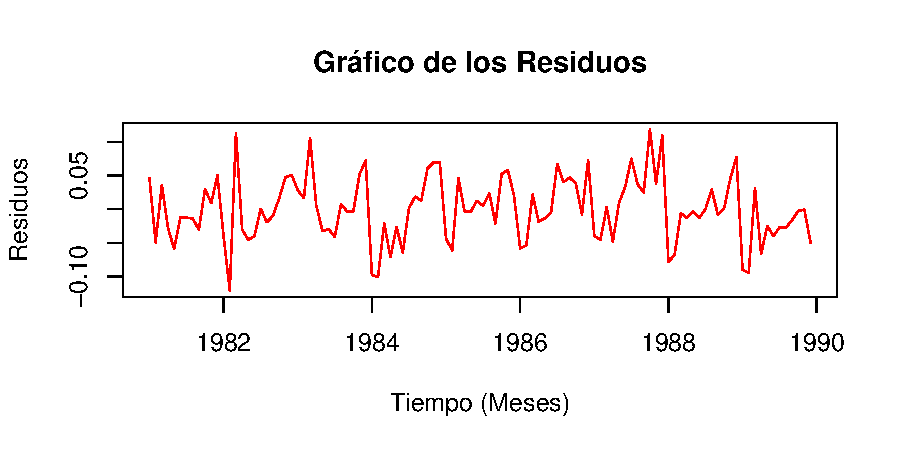
\includegraphics{Tarea-Empírica-2---Matías-Vicuña_files/figure-latex/Gráfico 2-1.pdf}

Continuación Respuesta: Al igual que en el gráfico de residuo de la
regresión anterior, este modelo tiene una media y una varianza no
constante, por lo que los efectos ciclicos que hay dentro de la muestra
no contemplan un punto medio, sino que aleatoriza los efectos que se
logran observar.

\hypertarget{pregunta-4}{%
\subsection{Pregunta 4}\label{pregunta-4}}

\% Table created by stargazer v.5.2.3 by Marek Hlavac, Social Policy
Institute. E-mail: marek.hlavac at gmail.com \% Date and time: Tue, Aug
30, 2022 - 23:55:23

\begin{table}[!htbp] \centering 
  \caption{} 
  \label{} 
\begin{tabular}{@{\extracolsep{5pt}}lc} 
\\[-1.8ex]\hline 
\hline \\[-1.8ex] 
 & \multicolumn{1}{c}{\textit{Dependent variable:}} \\ 
\cline{2-2} 
\\[-1.8ex] & log(totacc) \\ 
\hline \\[-1.8ex] 
 Constant & 10.63$^{***}$ \\ 
  & (0.08) \\ 
  trend(db\_ts) & 0.02$^{***}$ \\ 
  & (0.004) \\ 
  spdlaw & $-$0.06$^{***}$ \\ 
  & (0.02) \\ 
  beltlaw & 0.07$^{***}$ \\ 
  & (0.02) \\ 
  unem & $-$0.03$^{***}$ \\ 
  & (0.005) \\ 
  wkends & 0.01$^{**}$ \\ 
  & (0.005) \\ 
 \hline \\[-1.8ex] 
Observations & 108 \\ 
R$^{2}$ & 0.80 \\ 
\hline 
\hline \\[-1.8ex] 
\textit{Note:}  & \multicolumn{1}{r}{$^{*}$p$<$0.1; $^{**}$p$<$0.05; $^{***}$p$<$0.01} \\ 
\end{tabular} 
\end{table}

Respuesta: En la variable de \(spdlaw\) hay un efecto esperado, que es
al haberse aplicado esta ley, el porcentaje de accidentes disminuye un
6\% aproximadamente, pero, en el apartado de la variable \(beltlaw\) se
ve un efecto contrario, esto puede ser explicado de modo que, al ser
obligatorio el uso de accidentes, el efecto que se generó no fue si no
el que los conductores se sintieran más seguros a la hora de conducir, y
por lo mismo, generó una mayor irresponsabilidad al momento de las
precauciones al realizar la actividad, lo que genera un mayor porcentaje
de accidentes dada la aplicación de esta ley, concretamente, un 7\% más
aproximadamente.

\newpage

\hypertarget{pregunta-5}{%
\subsection{Pregunta 5}\label{pregunta-5}}

\% Table created by stargazer v.5.2.3 by Marek Hlavac, Social Policy
Institute. E-mail: marek.hlavac at gmail.com \% Date and time: Tue, Aug
30, 2022 - 23:55:24

\begin{table}[!htbp] \centering 
  \caption{} 
  \label{} 
\begin{tabular}{@{\extracolsep{5pt}}lc} 
\\[-1.8ex]\hline 
\hline \\[-1.8ex] 
 & \multicolumn{1}{c}{\textit{Dependent variable:}} \\ 
\cline{2-2} 
\\[-1.8ex] & prcfat \\ 
\hline \\[-1.8ex] 
 Constant & 1.03$^{***}$ \\ 
  & (0.14) \\ 
  trend(db\_ts) & $-$0.03$^{***}$ \\ 
  & (0.01) \\ 
  spdlaw & 0.08$^{**}$ \\ 
  & (0.03) \\ 
  beltlaw & $-$0.05 \\ 
  & (0.03) \\ 
  unem & $-$0.02$^{**}$ \\ 
  & (0.01) \\ 
  wkends & 0.01 \\ 
  & (0.01) \\ 
 \hline \\[-1.8ex] 
Observations & 108 \\ 
R$^{2}$ & 0.24 \\ 
\hline 
\hline \\[-1.8ex] 
\textit{Note:}  & \multicolumn{1}{r}{$^{*}$p$<$0.1; $^{**}$p$<$0.05; $^{***}$p$<$0.01} \\ 
\end{tabular} 
\end{table}

Respuesta: Ahora se logra ver que, al evaluar la variable \(prcfat\), el
efecto en \(spdlaw\) y \(beltlaw\) es totalmente diferente, esto se
explica dado que, a la hora de aplicarse la ley del cinturón, este trajo
consigo un efecto de disminución de accidentes en dónde hubiera al menos
un muerto, aproximadamente fue un 5\% de reducción de estos tipos de
accidentes dada la ley. En cambio, para la ley de velocidad máxima, el
efecto fue contrario, habiendo un aumento del 8\% de los accidentes con
al menos un fallecido al haberse aplicado esta ley.

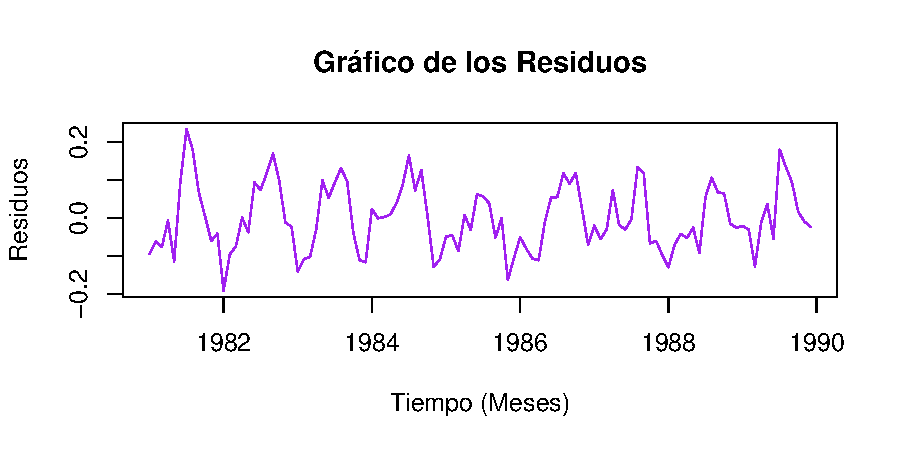
\includegraphics{Tarea-Empírica-2---Matías-Vicuña_files/figure-latex/regress 3-1.pdf}

Continuación Respuesta: Al igual que en las otras veces, se ve grandes
cambios ciclicos, pero esta vez con un efecto que gráficamente pareciera
seguir un patrón, se ve que hay un punto contemporáneo tal en cada año
en dónde los accidentes con al menos un fallecido tiene un incremento
dado los residuos del modelo.

\newpage

\hypertarget{pregunta-6}{%
\subsection{Pregunta 6}\label{pregunta-6}}

\% Table created by stargazer v.5.2.3 by Marek Hlavac, Social Policy
Institute. E-mail: marek.hlavac at gmail.com \% Date and time: Tue, Aug
30, 2022 - 23:55:24

\begin{table}[!htbp] \centering 
  \caption{} 
  \label{} 
\begin{tabular}{@{\extracolsep{5pt}}lc} 
\\[-1.8ex]\hline 
\hline \\[-1.8ex] 
 & \multicolumn{1}{c}{\textit{Dependent variable:}} \\ 
\cline{2-2} 
\\[-1.8ex] & log(totacc) \\ 
\hline \\[-1.8ex] 
 Constant & 10.47$^{***}$ \\ 
  & (0.02) \\ 
  season(db\_ts)Feb & $-$0.04$^{*}$ \\ 
  & (0.02) \\ 
  season(db\_ts)Mar & 0.08$^{***}$ \\ 
  & (0.02) \\ 
  season(db\_ts)Apr & 0.02 \\ 
  & (0.02) \\ 
  season(db\_ts)May & 0.03 \\ 
  & (0.02) \\ 
  season(db\_ts)Jun & 0.02 \\ 
  & (0.02) \\ 
  season(db\_ts)Jul & 0.04 \\ 
  & (0.02) \\ 
  season(db\_ts)Aug & 0.05$^{**}$ \\ 
  & (0.02) \\ 
  season(db\_ts)Sep & 0.04$^{*}$ \\ 
  & (0.02) \\ 
  season(db\_ts)Oct & 0.08$^{***}$ \\ 
  & (0.02) \\ 
  season(db\_ts)Nov & 0.07$^{***}$ \\ 
  & (0.02) \\ 
  season(db\_ts)Dec & 0.10$^{***}$ \\ 
  & (0.02) \\ 
  trend(db\_ts) & 0.03$^{***}$ \\ 
  & (0.002) \\ 
 \hline \\[-1.8ex] 
Observations & 108 \\ 
R$^{2}$ & 0.80 \\ 
\hline 
\hline \\[-1.8ex] 
\textit{Note:}  & \multicolumn{1}{r}{$^{*}$p$<$0.1; $^{**}$p$<$0.05; $^{***}$p$<$0.01} \\ 
\end{tabular} 
\end{table}

Respuesta: Al momento de realizar la regresión con las dummies de los
meses (descontando enero) y ajustando por tendendia, se observa que,
gran candidad de variables dummy (además de la tendencia) son
estadísticamente significativas, por lo cuál explican gran parte de los
efectos de la cantidad de accidentes que hay, a lo cuál se puede
concluir que si hay estacionalidad presente en el modelo que explica el
número de accidentes en cada época del año.

\end{document}
